\section{Introduction}
\label{sec:intro}

Given two untrimmed videos, video copy localization (VCL) asks which temporal intervals
depict the same content and returns the corresponding interval pairs. It underlies
near-duplicate removal, copyright triage, provenance analysis and attribution of re-uploaded
content~\cite{vcsl2022,transvcl2023}. The task is harder than whole-video retrieval: a copy
may occupy a small fraction of either video, may be re-encoded, cropped, overlaid or
speed-adjusted, and the answer must be expressed as start and end times on \emph{both} axes
rather than as a single similarity score.

Modern systems start from pre-extracted per-frame descriptors. Classical geometric and
alignment methods---Hough voting (HV), temporal networks (TN), dynamic programming (DP) and
dynamic time warping (DTW)---score frame pairs and search for a consistent monotone path,
without training a localization model~\cite{douze2016,jiang2014,tan2009,chou2015}. Learned
localizers either detect copied regions on a similarity map with a trained
detector~\cite{spd2021,vcsl2022}, or enhance frame features with self-/cross-attention and
regress boxes with a detection head~\cite{transvcl2023,rtr2024}; recent variants add regional
tokens, instance graphs or single-frame supervision~\cite{rtr2024,ding2025iesta,li2025vcsa}.
Both families have improved accuracy, and learned localizers currently report the strongest
numbers on public benchmarks~\cite{vcsl2022,figvcl2025}.

Their cost structure is less often discussed. A dense comparison evaluates a large part of
the $M\times N$ frame-pair product, where $M,N$ are feature-row counts; a
$1{,}000\times1{,}000$ pair already contains $10^6$ pairs of 256-dimensional descriptors.
Learned localizers reduce the constant and can process long inputs in chunks---TransVCL, for
example, splits features into $\le1{,}200$-frame blocks~\cite{transvcl2023}---but their cost
remains tied to dense in-chunk correlation or attention rather than to the number of copies
present. In practice, almost all frame pairs are irrelevant: a copy is a low-dimensional,
locally coherent structure in the time plane.

This suggests a structural question that, to our knowledge, has not been tested as an
independent hypothesis:

\begin{quote}
\emph{Must the coarse search that discovers candidate copies and the fine alignment that
determines their boundaries share the same dense computational domain?}
\end{quote}

We study a deliberately simple answer. If a small set of sparse, mutually consistent frame
correspondences is already concentrated around the true copy, it can \emph{propose} a few
finite regions of the time plane, and high-resolution alignment can be restricted to those
regions. The proposal stage is cheap and may miss things; the refinement stage is accurate
but can only act where a proposal exists. The scientific content is therefore not the cascade
itself---mutual nearest neighbours, RANSAC and banded dynamic programming are classical, and
RANSAC line fitting on the time plane is already standard in recent challenge matching
tracks~\cite{liu2023sam,pizzi2024vsc}---but the \emph{allocation of computation}, the failure
modes it creates, and whether those failures can be measured and controlled. Sampling
efficiency itself has been studied~\cite{chen2025sampling}; our question is whether coverage
and boundary refinement can be decoupled and measured separately, and where that decoupling
stops working.

\paragraph{What we do not claim.}
We do not claim that sparse proposals are sufficient, that finite tubes recover boundaries
better than a global path, or that the pipeline is faster on real hardware. Each is a
falsifiable hypothesis:

\begin{itemize}
\item \textbf{H1 (candidate coverage).} At substantially fewer frame-pair dot products, sparse
matching plus track fitting still covers true copies at high recall, including short copies.
\item \textbf{H2 (boundary recovery).} Zero-floored local alignment inside a finite tube
improves start/end boundaries over the coarse track support, rather than merely adding work.
\item \textbf{H3 (system benefit).} The saved fine-alignment domain converts into lower
end-to-end latency and memory on the same hardware, rather than being consumed by Python
loops, predecessor scans or data movement.
\end{itemize}
H1 can fail even if H2 holds (refinement cannot recover an uncovered copy), and H2 can hold
without H3 (a smaller domain is not a smaller wall-clock cost). We pre-register the
observations that would refute each one (Section~\ref{sec:exp}).

\paragraph{Contributions.}
The draft makes three contributions, stated conditionally because the empirical gate has not
been passed.
\begin{enumerate}
\item \emph{A specification and cost analysis of the sparse-to-tube decomposition.} We make
explicit what is computed on which domain and separate three notions that are often conflated:
not storing the full $M\times N$ matrix (memory), retaining few anchors (output sparsity), and
performing sub-quadratic arithmetic. Fixed-stride coarse matching remains $\Theta(MN)$; only
the constant and the memory footprint change. For refinement we distinguish the ideal
$O(LW)$ direct-offset dynamic program from the $O(PLW^2)$ cost of scanning a predecessor row
($L$ tube length, $W$ band width, $P$ paths).
\item \emph{A candidate mechanism with explicit counterexamples.} We formulate a zero-floored
finite-tube alignment, dual-axis support and gap splitting, and a minimum-IoU de-duplication
that preserves one-to-many copies. On hand-constructed inputs we show that replacing the zero
floor with unconditional continuation changes behaviour in two regimes---a long weak prefix
before a real copy, and two copies separated by a long weak gap---and we make this semantics
an experimental variable rather than a claimed improvement.
\item \emph{A comparison protocol designed to falsify the claim.} It fixes the feature
extractor, pair list, ground truth, evaluator and timing boundary; tunes each method's
threshold independently on validation; reports the four denominators the official macro
metric actually uses; measures negative-pair false alarms only on the split that contains
negatives; and includes a strong \emph{Simple Sparse-to-Band} baseline that already contains
every classical ingredient. If the pipeline does not beat that baseline at equal dot-product
budget, the mechanism increment is absent.
\end{enumerate}

\paragraph{Status of the evidence.}
This is a specification-and-protocol draft. The benchmark runs needed to fill the tables are
not complete, no test split has been scored, and no GPU timing exists. Every result cell in
Section~\ref{sec:exp} is marked \TODO{PENDING}. We deliberately do not fill those cells with
development runs, partial runs or synthetic numbers; Section~\ref{sec:exp-status} explains why
the existing diagnostics are not admissible. The supplementary material contains the
implementation audit, hyperparameters, metric details and the development-run status table.%
\footnote{``Fast'' is a project codename. No speed advantage is claimed anywhere in this
draft; the timing protocol is defined so that such a claim can be tested later.}

\begin{figure*}[t]
  \centering
  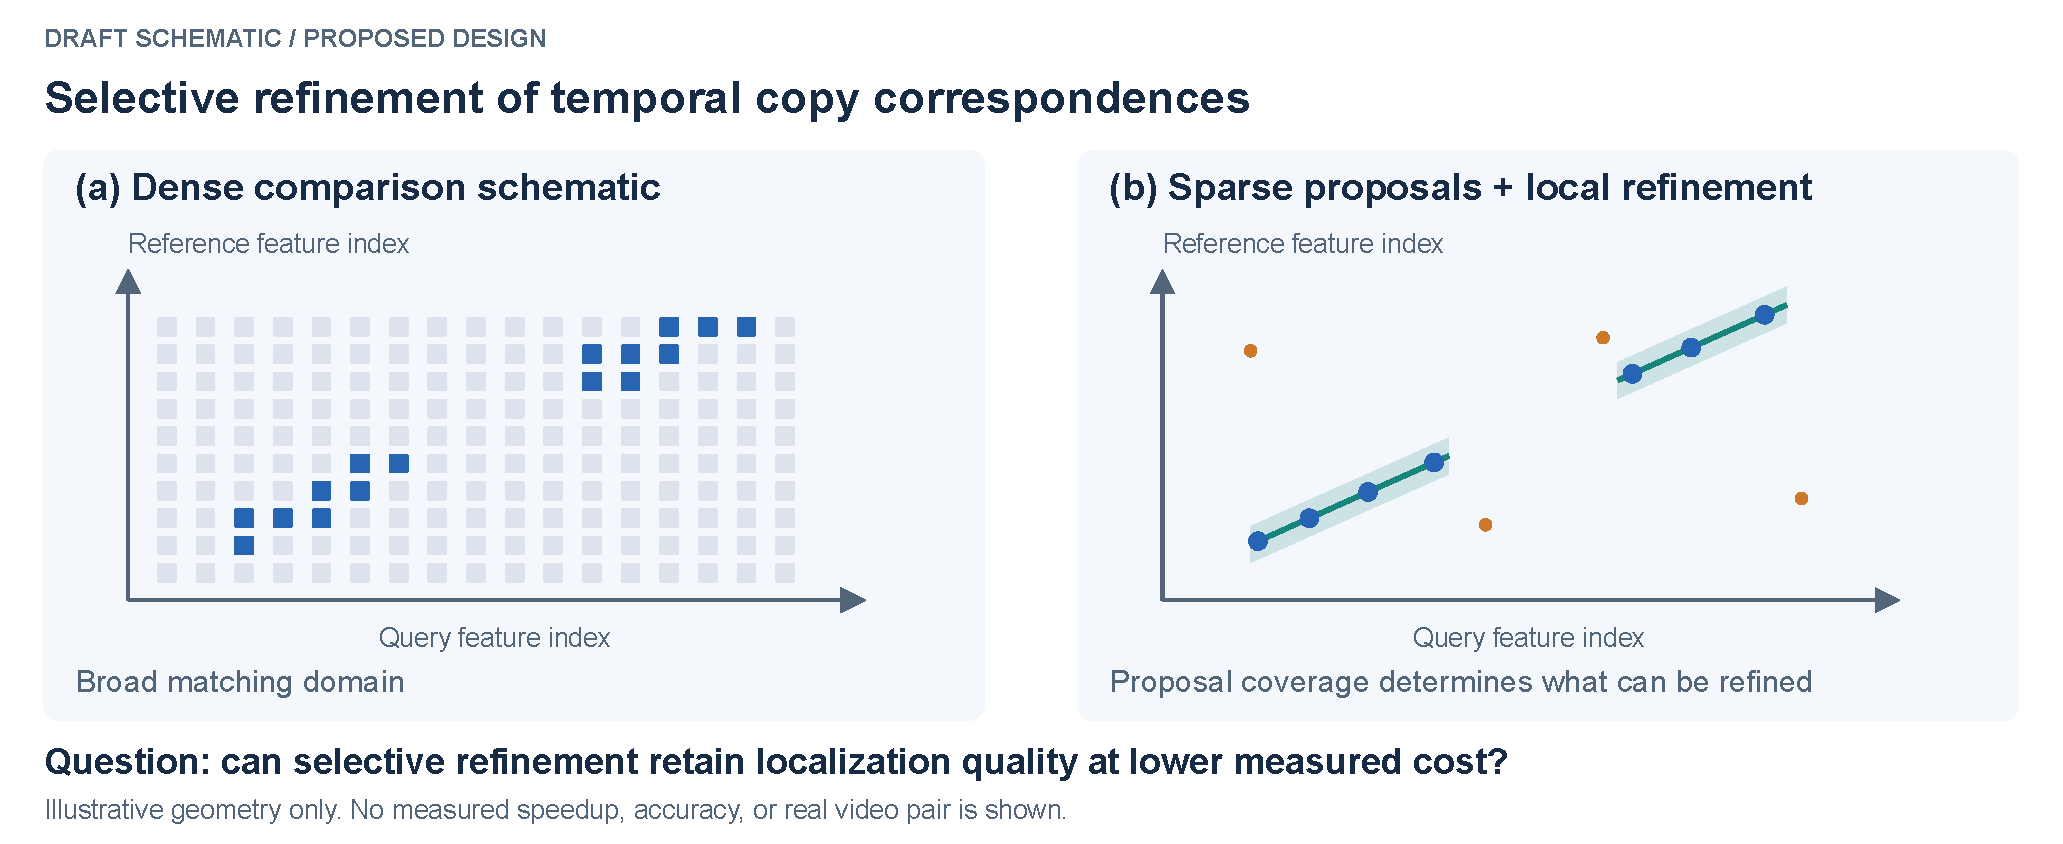
\includegraphics[width=0.86\textwidth]{figures/fig_1_teaser.pdf}
  \caption{\textbf{Conceptual comparison of matching domains.}
  (a) Dense comparison examines a broad frame-pair domain, of which only a few cells carry a
  copy. (b) Sparse temporal proposals restrict fine-resolution alignment to finite, locally
  supported regions. The geometry is illustrative (\emph{conceptual schematic}) and does not
  represent a measured baseline, a real video pair or an experimental output; the question at
  the bottom is the hypothesis tested here, not a result.}
  \label{fig:teaser}
\end{figure*}
